\documentclass[a4paper,12pt]{article}
\usepackage[utf8]{inputenc}
\usepackage[ngerman]{babel}
\usepackage[top=1in, bottom=1.25in, left=1.25in, right=1.25in]{geometry}
\usepackage{minted}
\usepackage{blindtext}
\usepackage{fancyhdr}
\usepackage{titling}
\usepackage{amssymb}
\usepackage{mathtools}
\usepackage{enumitem}
\usepackage{hyperref}
\usepackage{csquotes}
\MakeOuterQuote{"}

\hypersetup{colorlinks=true,linkcolor=blue,urlcolor=blue}

\renewcommand{\footrulewidth}{0.4pt}

\setlength\headheight{15pt}
\setlength{\parskip}{1em}

\title{GNS Aufgabe 2}
\author{Eli Kogan-Wang}
\date{\today}

\pagestyle{fancy}
\fancyhf{}
\lhead{\thetitle}
\rhead{\thedate}
\lfoot{\theauthor}
\rfoot{Page \thepage}


\begin{document}
% \maketitle
% \thispagestyle{fancy}

\section{Schauen Sie sich die folgenden Interfaces an}

Und identifizieren Sie, welche Laws of
UX und Gestalt Prinzipien benutzt werden, wie und wo sie benutzt werden, um was
zu erreichen. (Sie sollen hier keine Screenshots einfügen)

\begin{itemize}[label=a)]
  \item Audible Website:

        Eine Law, die auf jeden Fall verwendet wird ist: "Jakob’s Law", denn:

        Die Audible Website hat eine klassische Navigationsleiste, welche
        Links beim Hovern mit der Maus präsentieren. Auch präsentiert Audible eine Suchleiste
        oben rechts. Beide dieser Elemente sind auf vielen anderen Websites
        zu finden, und sind daher vertraut für den Benutzer.

        Eine andere Law, die verwendet wird ist "Tesler’s Law":

        Die Basiskomplexität der Kategorien-auswahl ist die Anzahl der Kategorien.
        Die Audible Website nimmt sogar schon eine Kategorisierung vor, indem
        Überkategorien gebildet und angezeigt werden. Der Nutzen kommt daher,
        dass der Benutzer nicht alle Kategorien durchsuchen muss, sondern
        nur die Überkategorien.

        Ein Gestalt Principle, dass verwendet wird ist "Similarity":

        Alle Kategorien-Links sind gleich dargestellt, da sie Instanzen
        derselben Interaktion darstellen.

        Zusätzlich sind die Kategorien-Links nah beieinander, sodass "Proximity"
        verwendet wird. Durch die nähe werden die Kategorien-Links gruppiert dargestellt,
        sodass man die bspw. von der Navbar darüber unterscheiden kann.

  \item National Geographic

        Eine Law, die auf jeden Fall verwendet wird ist: "Aesthetic-Usability Effect",
        denn die Website hat ein aesthetisches Design, durch die Verwendung von Bildern
        als Hintergrund und Interaktionselemente, sowie durch geometrische Anordnung. Dadurch
        wird die Website als benutzerfreundlicher wahrgenommen.

        Eine andere Law, die verwendet wird ist "Fitts’s Law": Die Interaktionselemente
        sind groß und nah beieinander, sodass sie leicht zu treffen sind. Die Interaktionselemente
        sind durch Bilder dargestellt, was ihre größe ermöglicht.

        Man verwendet auch das Gestalt Principle der "Symmetry and Order" indem die
        Hauptbedienelemente in einem symmetrischen Grid angeordnet sind. Dadurch
        wird die Ästhetik der Website verbessert.
\end{itemize}

\section{Machen Sie einen Screenshot}

Von einer beliebigen (arbeitssicheren) Schnittstelle
(kann auch PAUL, PANDA, UPB-Webseite, ... sein). (Bitte beachten Sie: Sie können
1 bis 4 Screenshots verwenden, um diese Frage zu beantworten)

% embed IMG_0094.jpg to IMTG_0096.jpg

\begin{figure}[h]
  \centering
  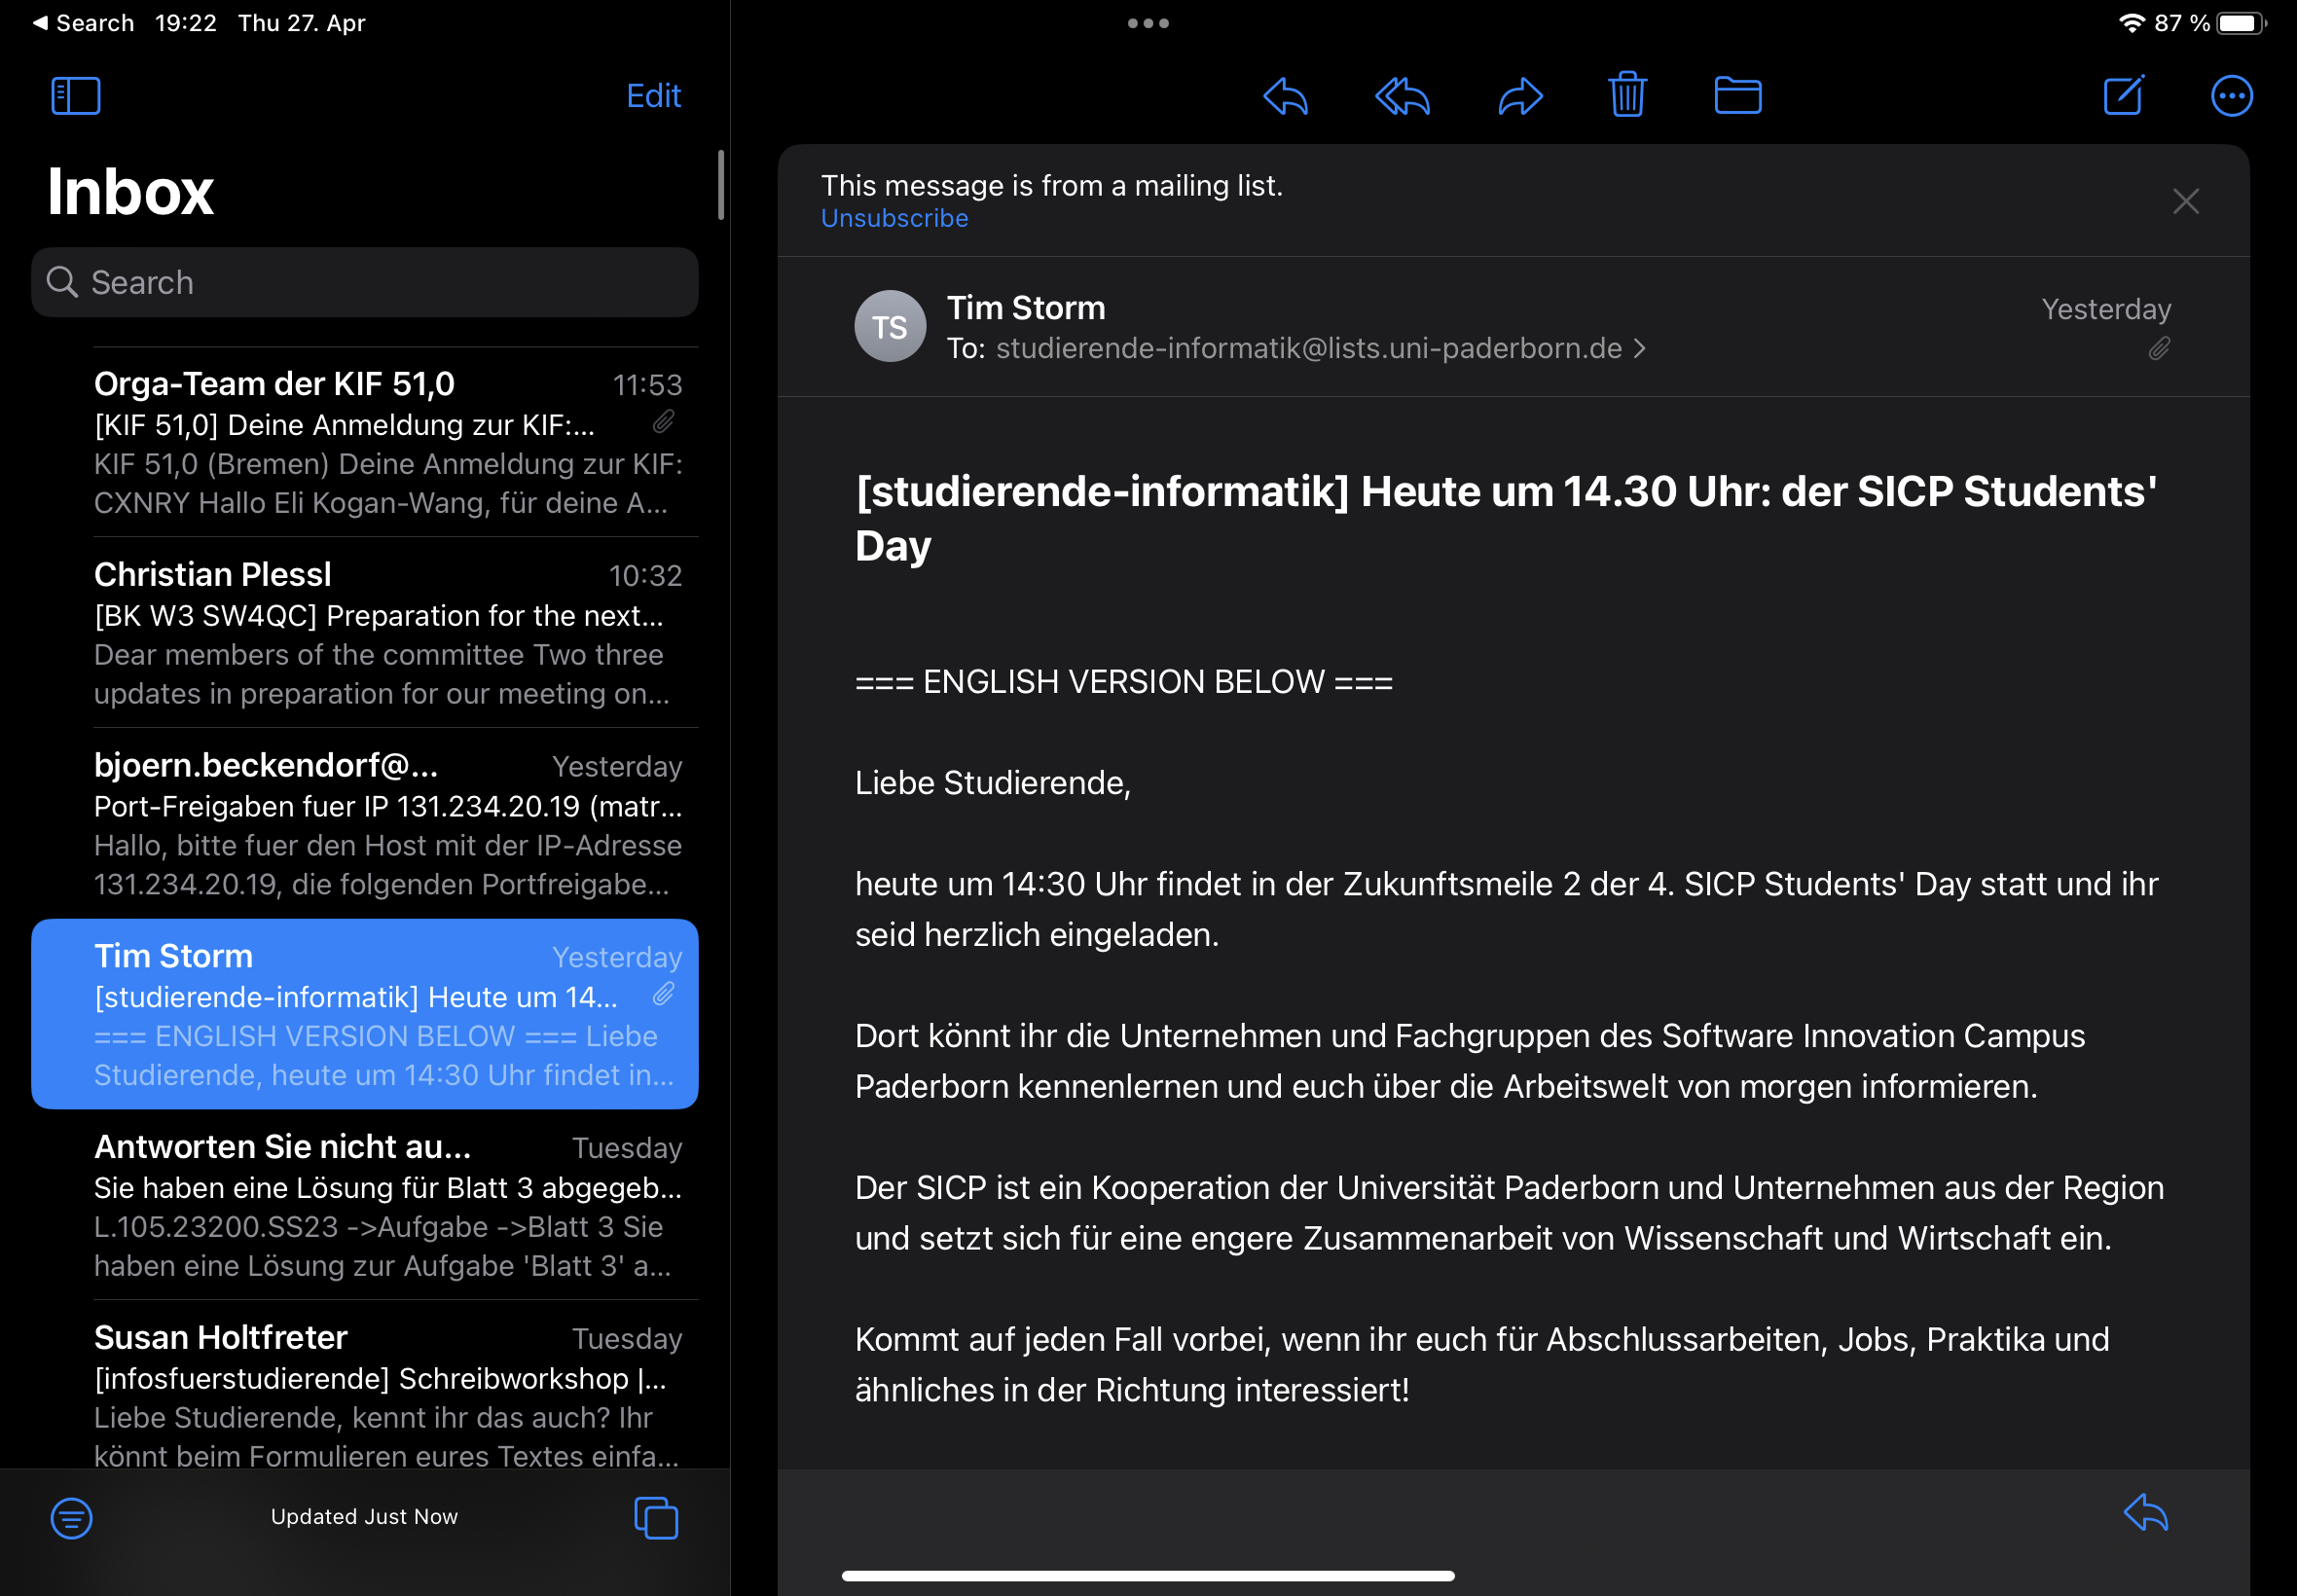
\includegraphics[width=0.8\textwidth]{IMG_0094.jpg}
  \caption{Screenshot von Apple Mail}
\end{figure}
\begin{figure}[h]
  \centering
  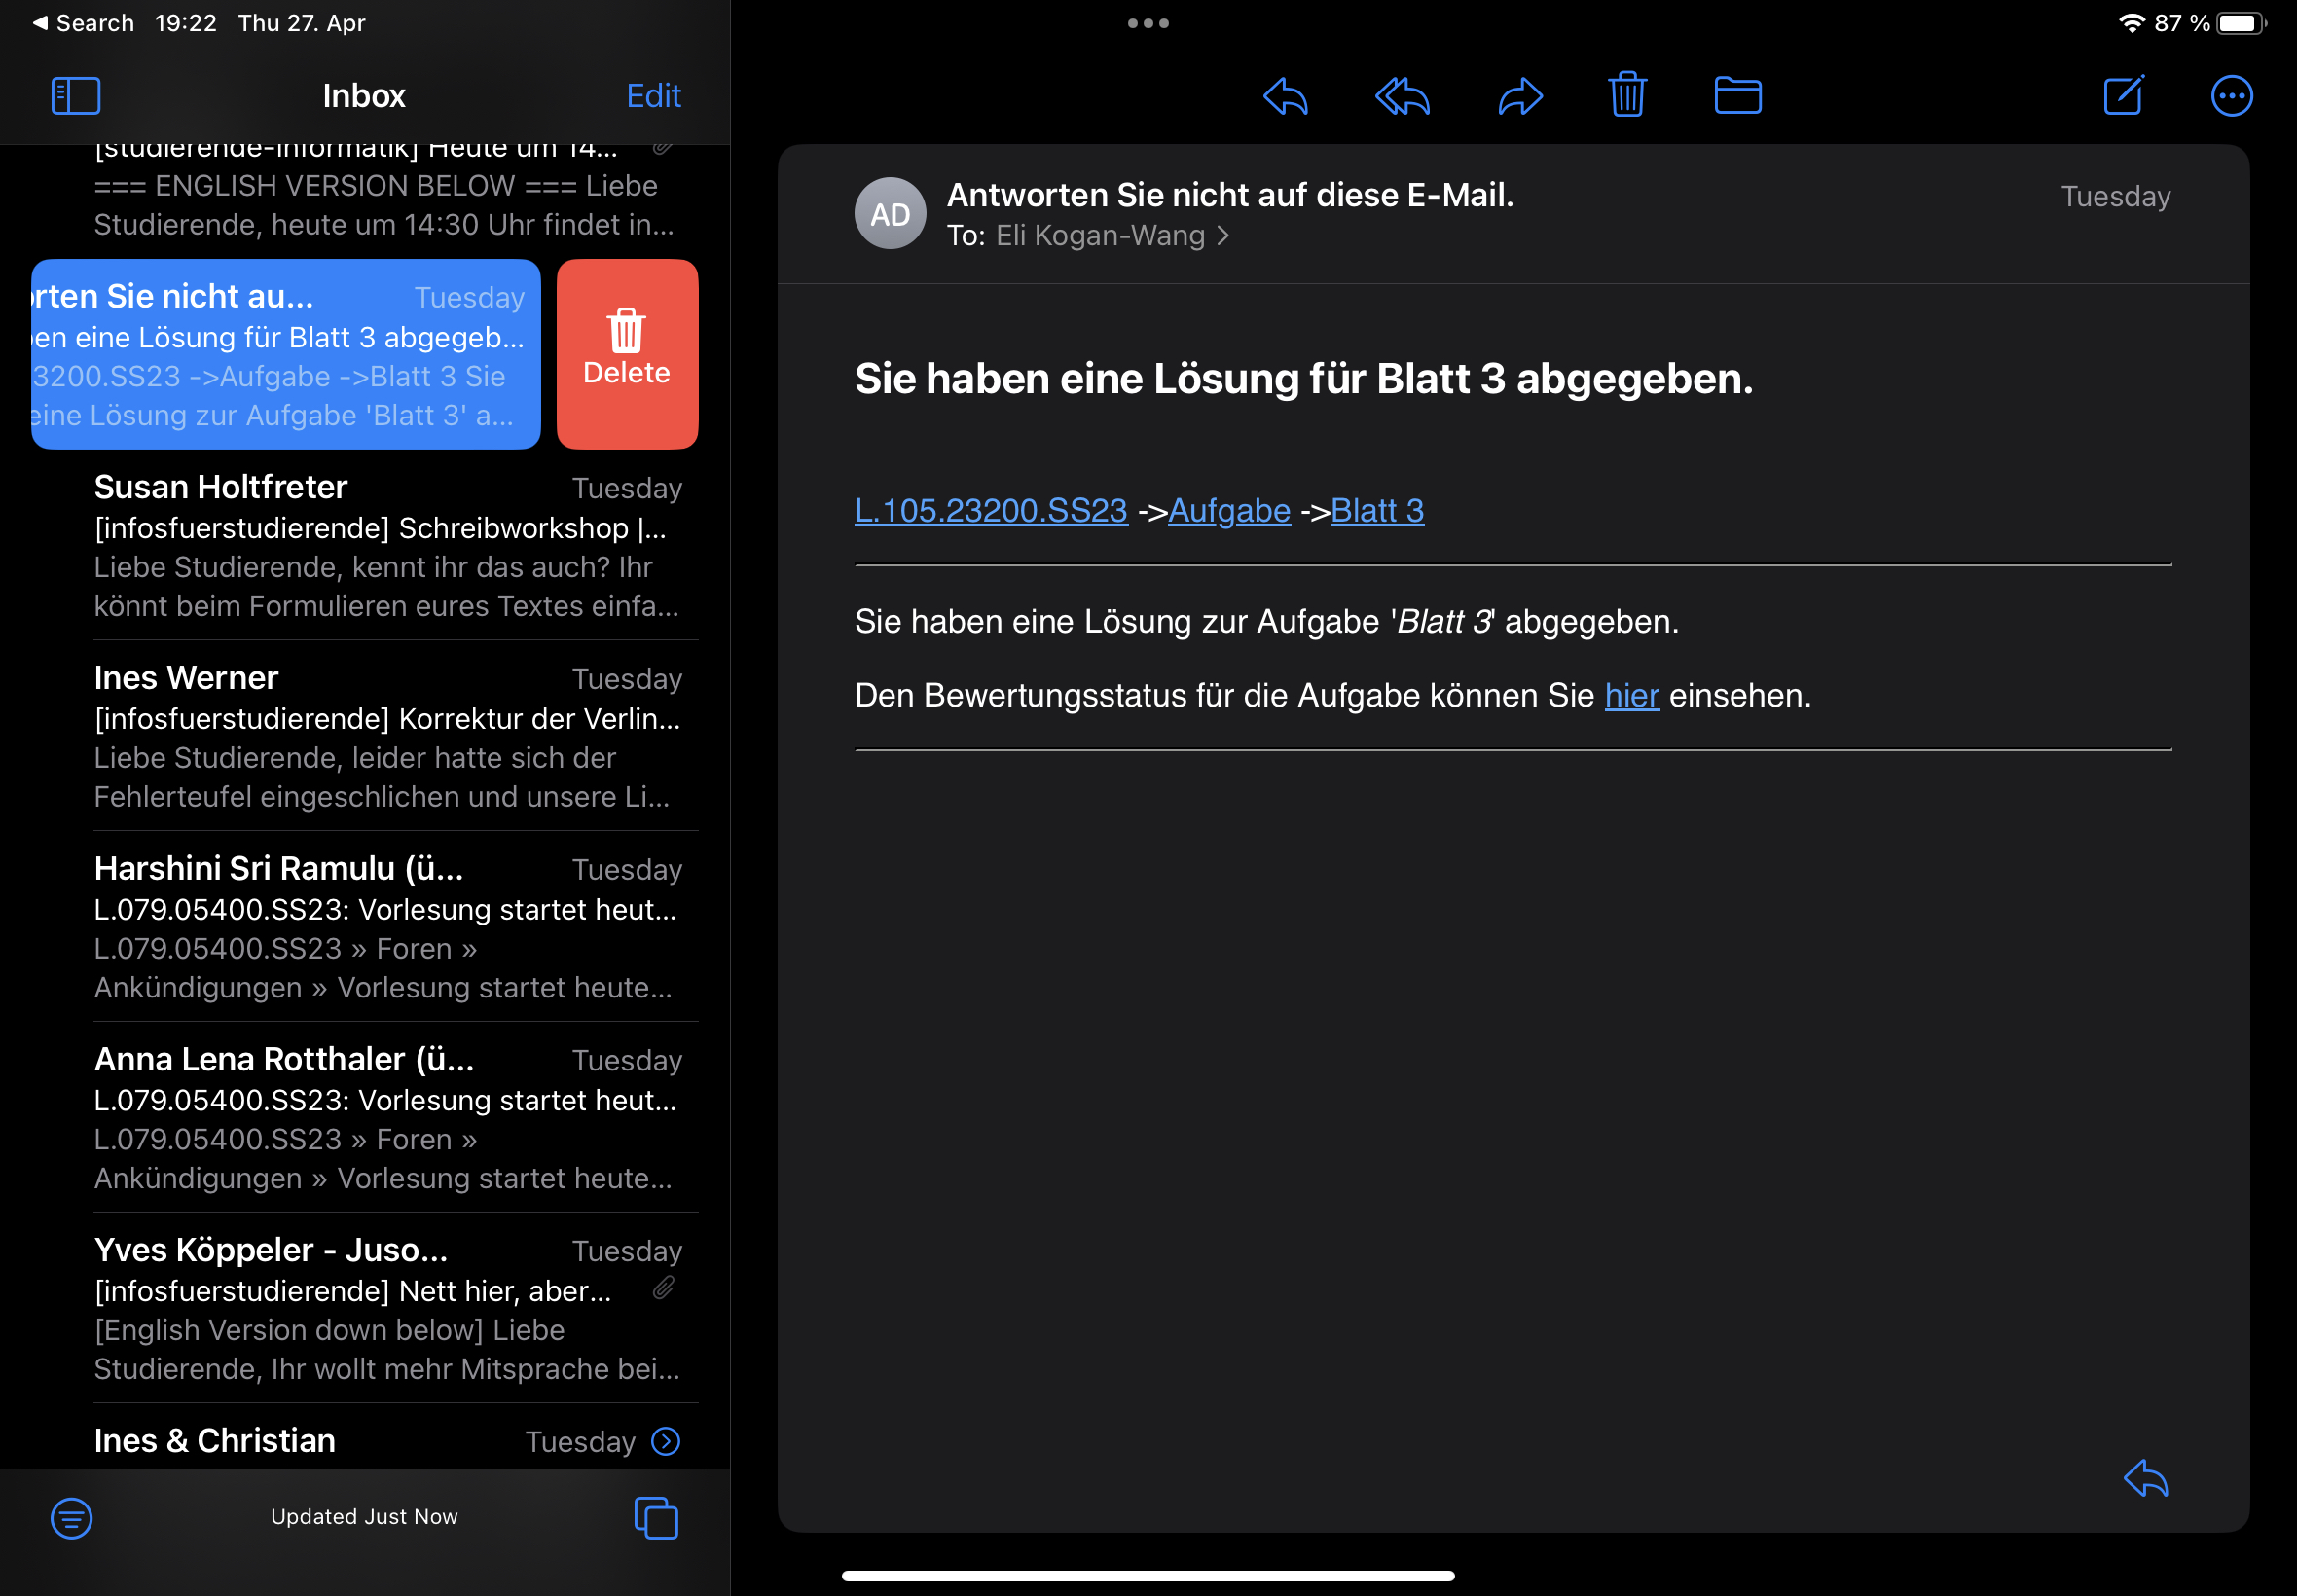
\includegraphics[width=0.8\textwidth]{IMG_0095.jpg}
  \caption{Screenshot von Apple Mail}
\end{figure}
\begin{figure}[h]
  \centering
  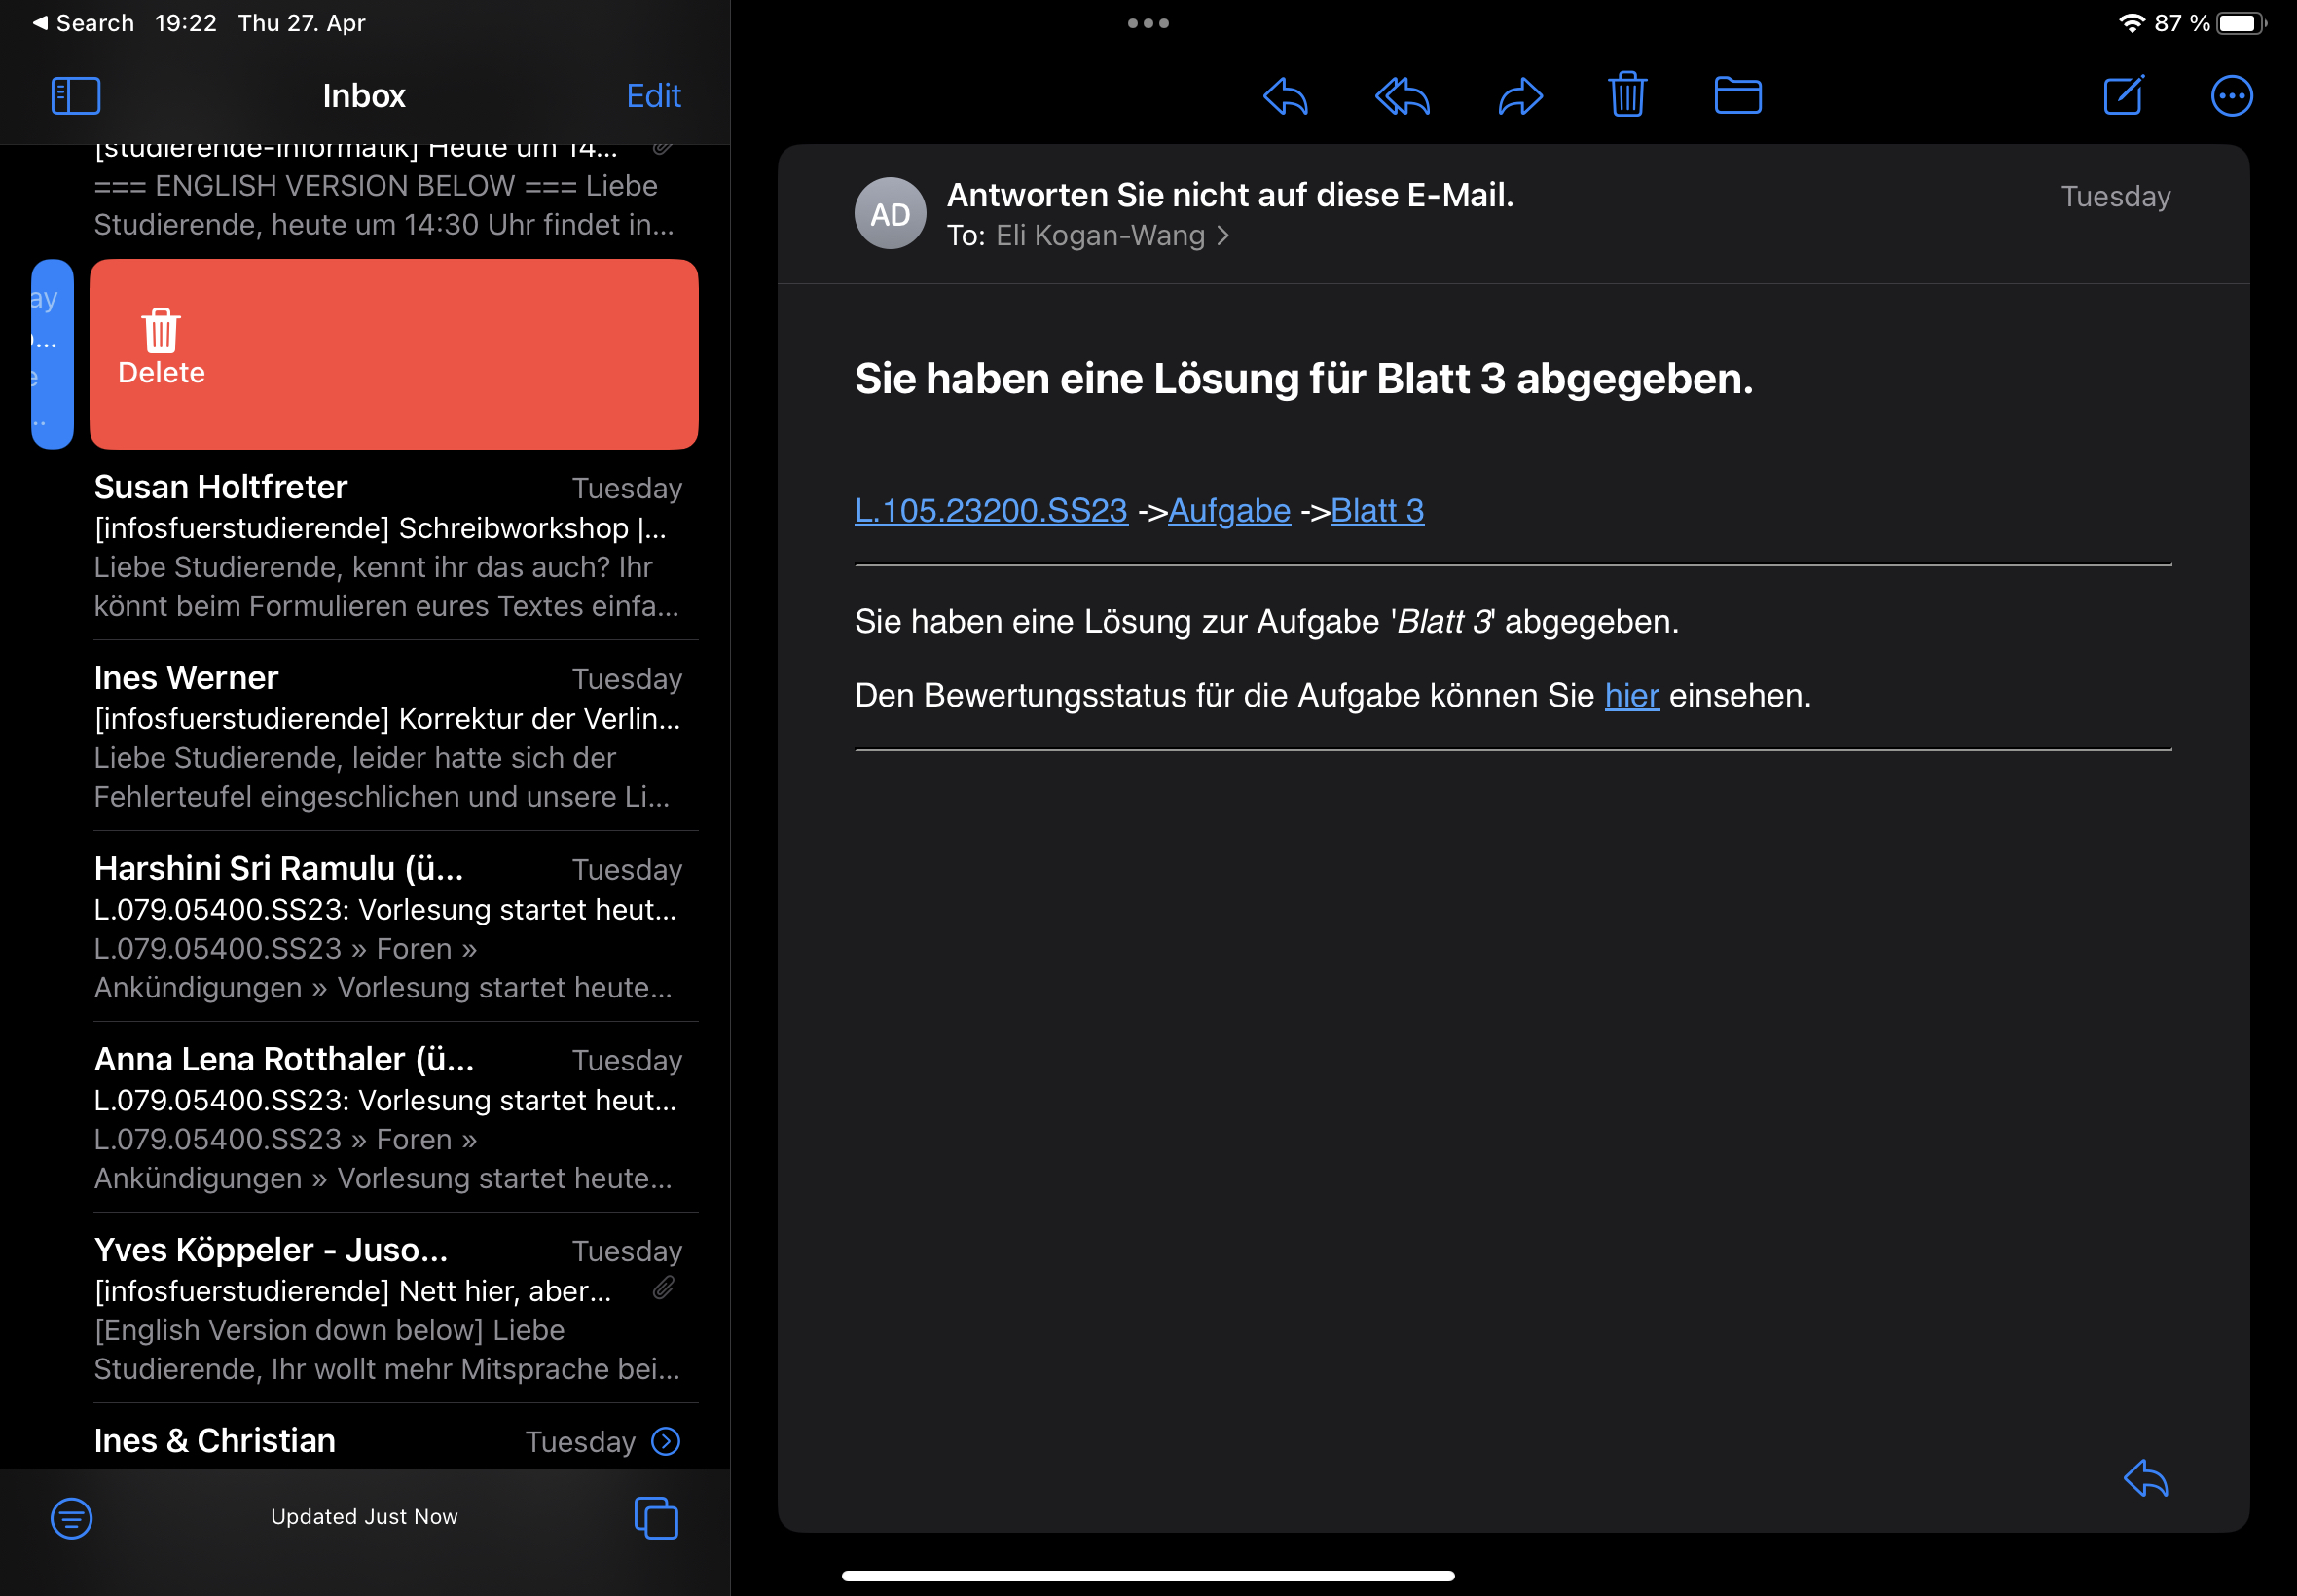
\includegraphics[width=0.8\textwidth]{IMG_0096.jpg}
  \caption{Screenshot von Apple Mail}
\end{figure}


Abgebildet ist eine Reihe von Screenshots von Apple Mail. Wir fokussieren
uns auf die Löschfunktion, die durch links-wischen aktiviert wird.

Diese Löschfunktion verletzt offensichtlich "Tesler's Law", da die Komplexität
der Funktion zu weit reduziert wurde, sodass die Funktion nicht mehr
sichtbar ist.

Für vorherige Nutzer von Desktop-Anwendungen (Ich) ist es auch eine Verletzung von "Jakob's Law",
da die Bedienweise "wische nach links um zu löschen" nicht vertraut ist.

Der "Goal-Gradient Effect" wird auch falsch verwendet, da die Löschfunktion
in der ersten und zweiten Zwischenansicht dem Nutzer keine Indikation darüber gibt, wie
nah er seinem Ziel (E-Mail löschen) angekommen ist. Der Button wird einfach länger.

Der "Zeigarnik Effect" wird auch falsch verwendet, da die Löschfunktion
keine Indikatoren liefert, dass sie existiert. Der Nutzer hat keine halb-vollständigen
Löschvorgänge auf dem Bildschirm, die darauf hindeuten, dass die Löschfunktion
existiert oder dass sie benutzt werden kann.

Mein Vorschlag ist folgender: Man entfernt die Lösch-durch-Wisch Funktion vollständig.
Die Funktionalität wird schon als mit Icon dargestellten Button dem Nutzer zur Verfügung
gestellt. Stattdessen kann man eine E-Mail-Management Funktion mit markieren von E-Mails
und Bulk-Funktionen also Massenlöschen, Massenarchivieren, etc. hinzufügen.

\end{document}
